\newpage
\section{Prinsipiell løsning}
\label{prinsipiellLoesning}

En differensialforsterker er en nøkkelkomponent i designet av operasjonsforsterkere (op-amp)\cite[s. 105]{Art of Eletronics}. I en differensialforsterker benyttes ofte to inngangstransistorer i en konfigurasjon som tillater differensiell signalbehandling. Bipolare transistorer, som for eksempel NPN- og PNP-transistorer, er valgt for deres egenskaper som forsterkningsenheter og deres evne til å drive signaler med høy presisjon. Et typisk eksempel på en differensialforsterker er vist i figur \ref{fig:diffamp}.

\begin{figure}[h]
    \centering
    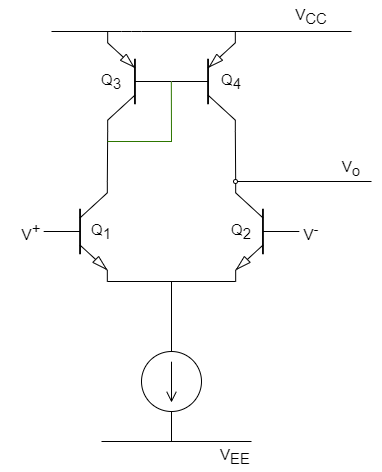
\includegraphics[width=0.6\textwidth]{Bilder/diffamp.drawio.png}
    \caption{Differensialforsterker som en operasjonsforsterker}
    \label{fig:diffamp}
\end{figure}

